\documentclass[AMS,STIX2COL]{WileyNJD-v2}

\articletype{Article Type}
\received{26 April 2016}
\revised{6 June 2016}
\accepted{6 June 2016}
\raggedbottom

\begin{document}
    \title{Transformer-Based Reranking \\for Improving Korean Morphological Analysis System}

    \author[1,2]{Jihee Ryu}
    \author[1]{Soojong Lim}
    \author[1]{Oh-Woog Kwon}
    \author[2]{Seung-Hoon Na*}
    \authormark{Jihee Ryu \textsc{et al}}

    \address[1]{\orgdiv{Language Intelligence Research Section}, \orgname{Electronics and Telecommunications Research Institute}, \orgaddress{\state{Daejeon}, \country{Republic of Korea}}}
    \address[2]{\orgdiv{Division of Computer Science and Engineering}, \orgname{Jeonbuk National University}, \orgaddress{\state{Jeollabuk-do}, \country{Republic of Korea}}}
    \corres{*Seung-Hoon Na, \orgdiv{Division of Computer Science and Engineering}, \orgname{Jeonbuk National University}, \orgaddress{\state{Jeollabuk-do}, \country{Republic of Korea}}. \email{nash@jbnu.ac.kr}}
    \presentaddress{Institute of Information \& Communications Technology Planning \& Evaluation(IITP) grant funded by the Korea government(MSIT) (RS-2023-00216011, Development of artificial complex intelligence for conceptually understanding and inferring like human)}

    \abstract[Abstract]{
        This study introduces a new approach in Korean morphological analysis, combining dictionary-based techniques with Transformer-based deep learning models.
        The key innovation is the use of a BERT-based Reranking system, significantly enhancing the accuracy of traditional morphological analysis.
        The methodology generates multiple suboptimal paths, then employs BERT models for reranking, leveraging their advanced language comprehension.

        Results show remarkable performance improvements, with the first-stage reranking achieving over 20\% improvement in Error Reduction Rate (ERR) compared to existing models.
        The second-stage, utilizing a different BERT variant, further increases this improvement in ERR to over 30\%.
        This indicates a significant leap in accuracy, validating the effectiveness of merging dictionary-based analysis with contemporary deep learning.

        The study suggests future exploration in refined integrations of dictionary and deep learning methods and using probabilistic models for enhanced morphological analysis.
        This hybrid approach sets a new benchmark in the field and offers insights for similar challenges in language processing applications.
    }
    \keywords{Korean morphological analysis, natural language understanding, deep learning, pretrained transformer encoder, reranking}

%    \JELinfo{classification}
%    \MSC{Code numbers}
    \jnlcitation{
        \cname{
            \author{Jihee Ryu},
            \author{Soojong Lim},
            \author{Oh-Woog Kwon},
            \author{Seung-Hoon Na}
        } (\cyear{2024}),
        \ctitle{Transformer-Based Reranking for Improving Korean Morphological Analysis System},
        \cjournal{ETRI Journal},
        \cvol{under review}.
    }

    \maketitle
%    \footnotetext{\textbf{Abbreviations:} ANA, anti-nuclear antibodies; APC, antigen-presenting cells; IRF, interferon regulatory factor}


    \begin{table*}[ht]
        \caption{Maximum performance of alternative paths as correct answers}
        \label{tab:maximum-performance}
        \centering
        \begin{tabular*}{500pt}{@{\extracolsep\fill}cccD{.}{.}{3}c@{\extracolsep\fill}}
            \toprule
            ~                 & \multicolumn{2}{@{}c@{}}{Written Language Evaluation Set} & \multicolumn{2}{@{}c@{}}{Spoken Language Evaluation Set}                  \\ \cmidrule{2-3} \cmidrule{4-5}
            alternative range & eojeol accuracy & average number of alternative           & \multicolumn{1}{@{}l@{}}{eojeol accuracy} & average number of alternative \\
            \midrule
            no alternative    & 96.36           & 1.0                                     & 92.54                                     & 1.0                           \\
            secondary         & 98.74           & 25.7                                    & 97.27                                     & 12.9                          \\
            tertiary          & 98.96           & 47.8                                    & 97.81                                     & 23.6                          \\
            quarternary       & 99.01           & 69.6                                    & 97.95                                     & 34.2                          \\
            quinary           & 99.02           & 91.1                                    & 98.01                                     & 44.5                          \\
            \bottomrule
        \end{tabular*}
        \begin{tablenotes}
            \footnotesize
            \item\hspace{2mm} * Written Language Evaluation Set: 2,400 sentences each randomized from UCorpus and Everyone's Corpus (4,800 sentences total)
            \item\hspace{2mm} * Spoken Language Evaluation Set: 2,400 sentences each randomized from UCorpus and Everyone's Corpus (4,800 sentences total)
        \end{tablenotes}
    \end{table*}

    \section{Introduction}\label{sec:intro}

    Korean morphological analysis involves determining parts of speech by identifying morphemes, the smallest units of linguistic expression with independent meanings in a sentence.
    Unlike isolating languages like English, where sequential tagging suffices, Korean, being agglutinative, requires separating endings or postpositions and restoring inflections.
    The accuracy of morphological analysis significantly impacts Korean analysis performance since many tasks rely on separate morphemes as their basic input.
    Modern deep learning methods in natural language processing use tokenization, breaking text into smaller units and converting each into a vector for computational models~\cite{Mikolov2013}.
    For Korean, where subword units are crucial, attempting tokenization with separate morphemes in advance reflects the language's characteristics~\cite{SongHJ2021}.
    Incorporating morphological analysis results into this process enhances overall performance, capturing the semantic units of Korean.
    To accomplish this, we need a morphological analyzer that is not only highly accurate but also operates swiftly.

    Several approaches have been suggested for morphological analysis, a critical aspect of Korean language comprehension~\cite{KwonHC1991, LeeDG2009, ShimKS2011, LeeJS2011, ShinJC2012, LeeCK2013, NaSH2014, NaSH2015, HwangHS2016, KimHM2016, ChungES2016, LeeCH2016, Li2017, NaSH2018, KimSW2018, ChoiYS2018, MinJW2018, MinJW2019, KimHM2019, SongHJ2019, MinJW2020, SongHJ2020, ChoiYS2020, HwangHS2020, KimHJ2021, YounJY2021, MinJW2022, KimJM2022, ShinHJ2023}.
    Typically, when individuals grasp spoken or written language, they try to comprehend it through familiar vocabulary and concepts.
    While some approaches rely on rules or dictionaries to capture this understanding~\cite{KwonHC1991}, constructing and updating dictionaries for varied text vocabularies can be challenging.
    As a result, methods focusing on tagging syllable units without a dictionary have been proposed~\cite{ShimKS2011, LeeCK2013, LeeCH2016, KimHM2016} and studied for enhancement~\cite{KimSW2018, ChoiYS2018, KimHM2019, MinJW2019, SongHJ2019, SongHJ2020, YounJY2021, ShinHJ2023}.
    Mechanically, syllable-by-syllable morphological analysis can be achieved by either tagging syllables and then applying a base-form restoration dictionary~\cite{ShimKS2011, LeeCH2016} or by tagging syllables with the base form pre-restored~\cite{YounJY2021}.
    %However, this approach has limitations, struggling with precise morpheme boundary identification and struggling to grasp long-term contextual information as the sequence lengthens.
        However, this approach has limitations, struggling with identifying precise morpheme boundary identification and grasping long-term contextual information as the sequence lengthens.
    In this study, the former is termed dictionary-based morphological analysis, and the latter is syllable-unit morphological analysis.
    Both methods are trained on manually labeled corpora, facing challenges in accurately analyzing new syllable combinations or morphemes absent in the training data.
    The evolution of the Internet, open sources, and shared knowledge has led to substantial accumulations of web texts, corpora, language resources, offering an opportunity to overcome the constraints of dictionary-based methods due to reduced costs in dictionary construction and maintenance.

    Given this context, our study aims to enhance the effectiveness of the dictionary-based morphological analysis method employed by MeCab~\cite{MeCab}, an open-source tool for Korean and Japanese morphological analysis commonly used as a crucial preprocessing tool for deep learning.
    The method, trained through Conditional Random Fields (CRF), generates a lattice structure from a given sentence, connecting candidate morphemes in the dictionary through a directed graph.
    Subsequently, the optimal morphological analysis path is determined within this lattice structure~\cite{Kudo2004, NaSH2014, NaSH2018}.
    The Viterbi algorithm is employed in this process, minimizing the cost associated with each morpheme node and the sum of neighborhood costs for consecutive morphemes to identify the optimal path.

    In these dictionary-based morphological analysis methods, the primary errors stem from encountering new words absent in the dictionary within a sentence or when biases lead to the selection of an incorrect result during optimal path calculation.
    For instance, opting for one long morpheme over several short ones might be cost-effective but often results in an inaccurate analysis.
    The main impetus behind our study is the recognition that the path minimizing costs for nodes and links may not always align with the optimal path.
    In response, we propose methods to address these challenges and improve the accuracy of the morphological analysis process.

    \begin{figure*}[ht]
        \centerline{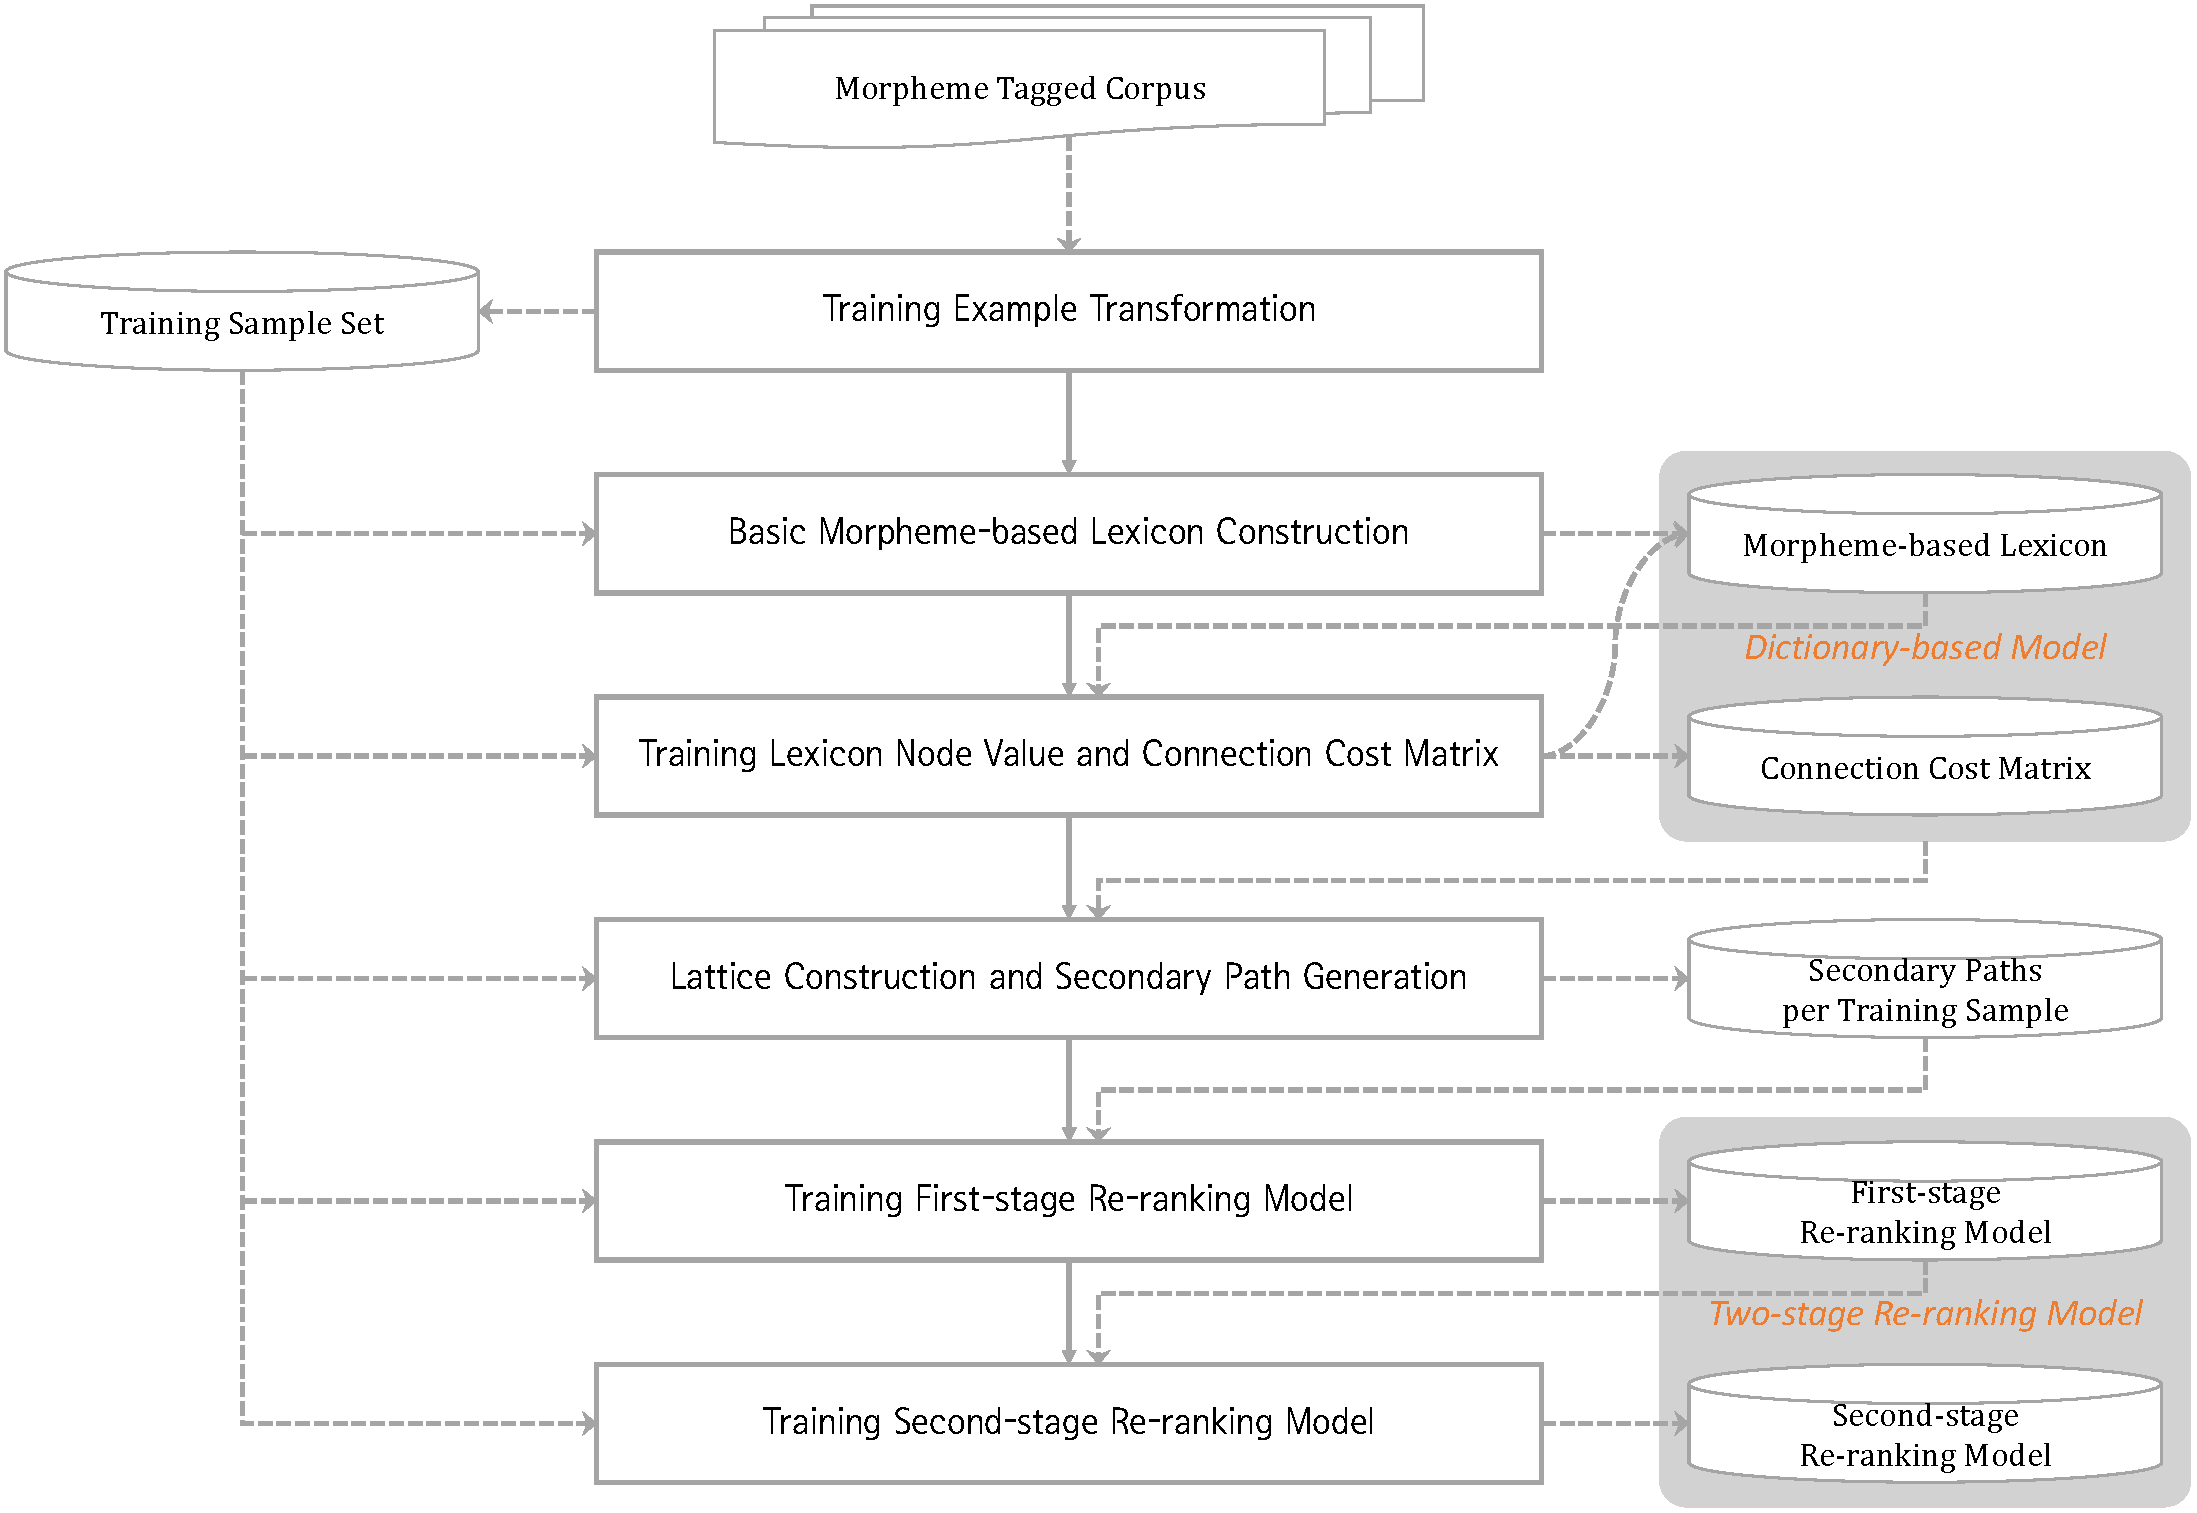
\includegraphics[width=1.0\textwidth]{fig;block-v1}}
        \caption{Overall process flow of the proposed method. Given morpheme-tagged corpus which consists of pairs of sentences and their morpheme-annotated results (in Section~\ref{subsec:korean-morphological-analysis-corpora}), the corpus preprocessing transforms a morpheme-tagged sentence into a training instance by performing the string alignment between its surface and lemma forms (in Section~\ref{subsec:training-example-transformation}). Under the transformed training corpus, the dictionary-based morphological analysis model is trained using the CRF algorithm, thereby constructing morpheme-based lexicon and obtaining lexicon node values and the connection cost matrix which are used to score a morphologinal analysis path (in Section~\ref{subsec:training-example-transformation}). Restricting possible paths by the morpheme-based lexicon, we construct a lattice, which compactly represents all possible paths based on a graph of nodes, where a connected path including the starting and ending nodes is considered as a morphological analysis path (in Section~\ref{subsec:lattice-construction-and-decoding}). For reranking, we generate secondary paths by alternatively replacing the top nodes in the optimal path by the next-top nodes (i.e. the secondary nodes) (in Section~\ref{subsec:secondary-path-generation}). Once a set of secondary paths is produced, we further apply two-stage reranking methods that 1) first performs the BERT-based reranking over a set of secondary paths (in Section~\ref{subsec:bert-based-reranking}) and then 2) carries out the additional reranking module applied on the concatenated input of a reranked path and an original input sentence (in Section~\ref{subsec:two-stage-reranking}).}
        \label{fig:block}
    \end{figure*}

    To pinpoint instances where a suboptimal solution may, in fact, be the best choice according to the best path calculation, we modified the best path calculation method to yield suboptimal analysis results and assessed their accuracy.
    While various approaches exist for selecting the next-best path, we opted for the method of substituting a morpheme node on the optimal path with a lower-ranked node.
    Table~\ref{tab:maximum-performance} illustrates the degree to which analysis performance can be enhanced by replacing the optimal path with a lower-ranked node.
    This problem is analogous to the challenge of reranking search results in information retrieval~\cite{BaeYJ2021}, where the goal is to identify the correct answer among the generated suboptimal results.

    In ~\cite{ChoiYS2018}, the N-best analysis results produced by the seq2seq model were reranked based on a convolutional neural network to enhance performance.
    In our study, we employed reranking with two distinct BERT models, each of different types and forms, as proposed in ~\cite{Nogueira2019}.
    Experimental results reveal that first-stage reranking improves performance by over 20\% compared to existing written and spoken models.
    Furthermore, second-stage reranking, incorporating a different input type and a diverse pre-trained model, contributes to a performance improvement exceeding 30\% compared to existing written and spoken models.

    While our introduced method led to further enhancement in the performance of the dictionary-based morphological analysis, it resulted in an overall increase in analysis time when configuring the morphological analysis system, including the reranking model itself.
    However, a promising avenue for future exploration lies in utilizing the results of multiple reranked morpheme analyses to update the connection costs between morphemes in a dictionary, akin to the backpropagation process in a typical neural network.
    It is anticipated that an improved morphological analysis system with updated connection costs can generate superior reranking candidates, potentially enabling iterative performance improvements.
    While this study focused on two-stage reranking, further research is essential to fully explore this potential.

    \begin{table*}[ht]
        \centering
        \footnotesize
        \caption{Statistics for the Korean morphological corpus as a whole and for training/test data}
        \label{tab:data-statistics}
        \begin{tabular}{m{20mm}m{14mm}m{10mm}m{12mm}m{10mm}m{10mm}m{12mm}m{10mm}m{10mm}m{12mm}m{10mm}}
            \toprule
            \multirow{2}{*}{Corpus}            & \multirow{2}{*}{Style} & \multicolumn{3}{c}{Raw Data}                 & \multicolumn{3}{c}{Training Data}            & \multicolumn{3}{c}{Test Data}             \\
            \cmidrule(lr){3-5} \cmidrule(lr){6-8} \cmidrule(lr){9-11}
            ~                                  & ~                      & sentences & eojeols    & morphs\newline/sent & sentences & eojeols    & morphs\newline/sent & sentences & eojeols & morphs\newline/sent \\
            \midrule
            Sejong Corpus                      & written                & 854,475   & 10,052,869 & 26.8                & 194,822   & 2,681,582  & 31.0                & 49,922    & 678,578 & 30.6                \\
            \midrule
            \multirow{3}{*}{UCorpus}           & written                & 5,456,101 & 62,462,158 & 25.1                & 4,998,560 & 57,393,332 & 25.4                & 53,003    & 598,413 & 25.0                \\
            ~                                  & semi-spoken            & 393,770   & 3,401,444  & 18.4                & 334,061   & 2,960,146  & 19.4                & 38,960    & 332,285 & 18.6                \\
            ~                                  & spoken                 & 627,380   & 2,819,427  & 10.9                & 429,215   & 2,295,940  & 13.0                & 62,399    & 279,545 & 11.1                \\
            \midrule
            \multirow{2}{*}{Everyone's Corpus} & written                & 150,082   & 2,000,213  & 30.4                & 129,352   & 1,713,367  & 30.5                & 14,442    & 191,223 & 30.5                \\
            ~                                  & spoken                 & 221,371   & 1,006,287  & 8.7                 & 137,869   & 714,021    & 10.5                & 19,789    & 85,316  & 8.6                 \\
            \bottomrule
        \end{tabular}
    \end{table*}

    The primary contributions of this study can be summarized as follows:
    \begin{enumerate}
        \item \textbf{Further improvement of dictionary-based morphological analysis method using suboptimal analysis results}: We investigate the potential for performance improvement by introducing a method to replace some nodes in the optimal path with suboptimal ones. Additionally, we propose an effective approach to enhance the dictionary-based morphological analysis method through deep learning.
        \item \textbf{Extending the performance improvement by introducing a two-stage reranking model}: To further enhance the performance of dictionary-based analysis through reranking, we suggest extending the improvement using different BERT models and conducting two rounds of reranking.
        \item \textbf{A method for updating connection costs in the dictionary and suggestions for future research}: We present a novel method for updating dictionary connection costs based on reranked morphological analysis results. Furthermore, we outline directions for future research, suggesting potential enhancements.
    \end{enumerate}
    These contributions provide valuable insights into advancing the performance of Korean morphological analysis and offer guidance for future researchers.

    The subsequent sections of this paper are organized as follows:
    Section ~\ref{sec:morphological-analysis-model} discusses the configuration and training of a dictionary-based morphological analysis system.
    Section ~\ref{sec:reranking-model} covers the generation of secondary results of morphological analysis, the production of reranking data, and the proposal of a method for training a two-stage reranking model.
    Section ~\ref{sec:results} delves into the results of the performance improvement using morphological analysis and reranking models.
    Section ~\ref{sec:related-work} introduces previous research cases related to this study.
    Finally, in Section ~\ref{sec:conclusion}, we conclude the study, discuss its limitations, and suggest directions for future research.


    \section{Morphological Analysis Model}\label{sec:morphological-analysis-model}

    Our proposed method for enhancing Korean morphological analysis involves integrating a Transformer-based reranking model into a dictionary-based morphological analysis system.
    Our approach is depicted in Figure~\ref{fig:block}, which illustrates the overall process flow.
    This section details the configuration and training of a dictionary-based morphological analysis system.

    \subsection{Korean Morphological Analysis Corpora}\label{subsec:korean-morphological-analysis-corpora}

    In this study, three major corpora were utilized to train and evaluate Korean morphological analysis models, each serving distinct research purposes and possessing unique characteristics:

    \textbf{Sejong Corpus}: Originating from the 21st Century Sejong Project, this corpus comprises a total of 15 million eojeols, including the raw untagged corpus~\cite{ChoeMW2008}.
    It forms the backbone of Korean morphological analysis research, offering a diverse array of linguistic patterns and structures crucial for baseline training and validation of morphological analysis models.
    The Sejong Corpus has been widely used for performance comparisons with other studies.
    For our experiments, we utilized the dataset used by researchers of ~\cite{MinJW2019, MinJW2020, MinJW2022, MinJW2018, NaSH2015, NaSH2014, NaSH2018, SongHJ2019, SongHJ2020}.

    \textbf{UCorpus (University of Ulsan Corpus)}~\cite{UCorpusHG}: An extension of the Sejong corpus, the UCorpus is continually maintained and expanded by the University of Ulsan.
    It has significantly grown in volume, reaching 63 million eojeols.
    This extension tests the adaptability and accuracy of the model across a broader range of data.
    Corrections to previously identified errors ~\cite{KimIH2010} and additional annotations for new data contribute to its value, providing a comprehensive basis for linguistic analysis.

    \textbf{Everyone's Corpus}~\cite{EveryoneCorpus}: Launched by the National Institute of the Korean Language in 2020, the Everyone's Corpus enriches the data landscape with contemporary web texts and spoken language materials~\cite{KimIH2019}.
    This modern corpus reflects the dynamic evolution of the Korean language, playing a pivotal role in improving models to capture the nuances of current Korean usage.

    Table~\ref{tab:data-statistics} presents specific details regarding the number of sentences and words in each corpus, along with the data subsets used for model training and evaluation.
    In the process of converting training data, we initially removed duplicate sentences and excluded those with annotation errors or other issues.
    Notably, a substantial occurrence of duplicate sentences was observed, particularly in spoken language datasets.

    \begin{figure*}[ht]
        \centerline{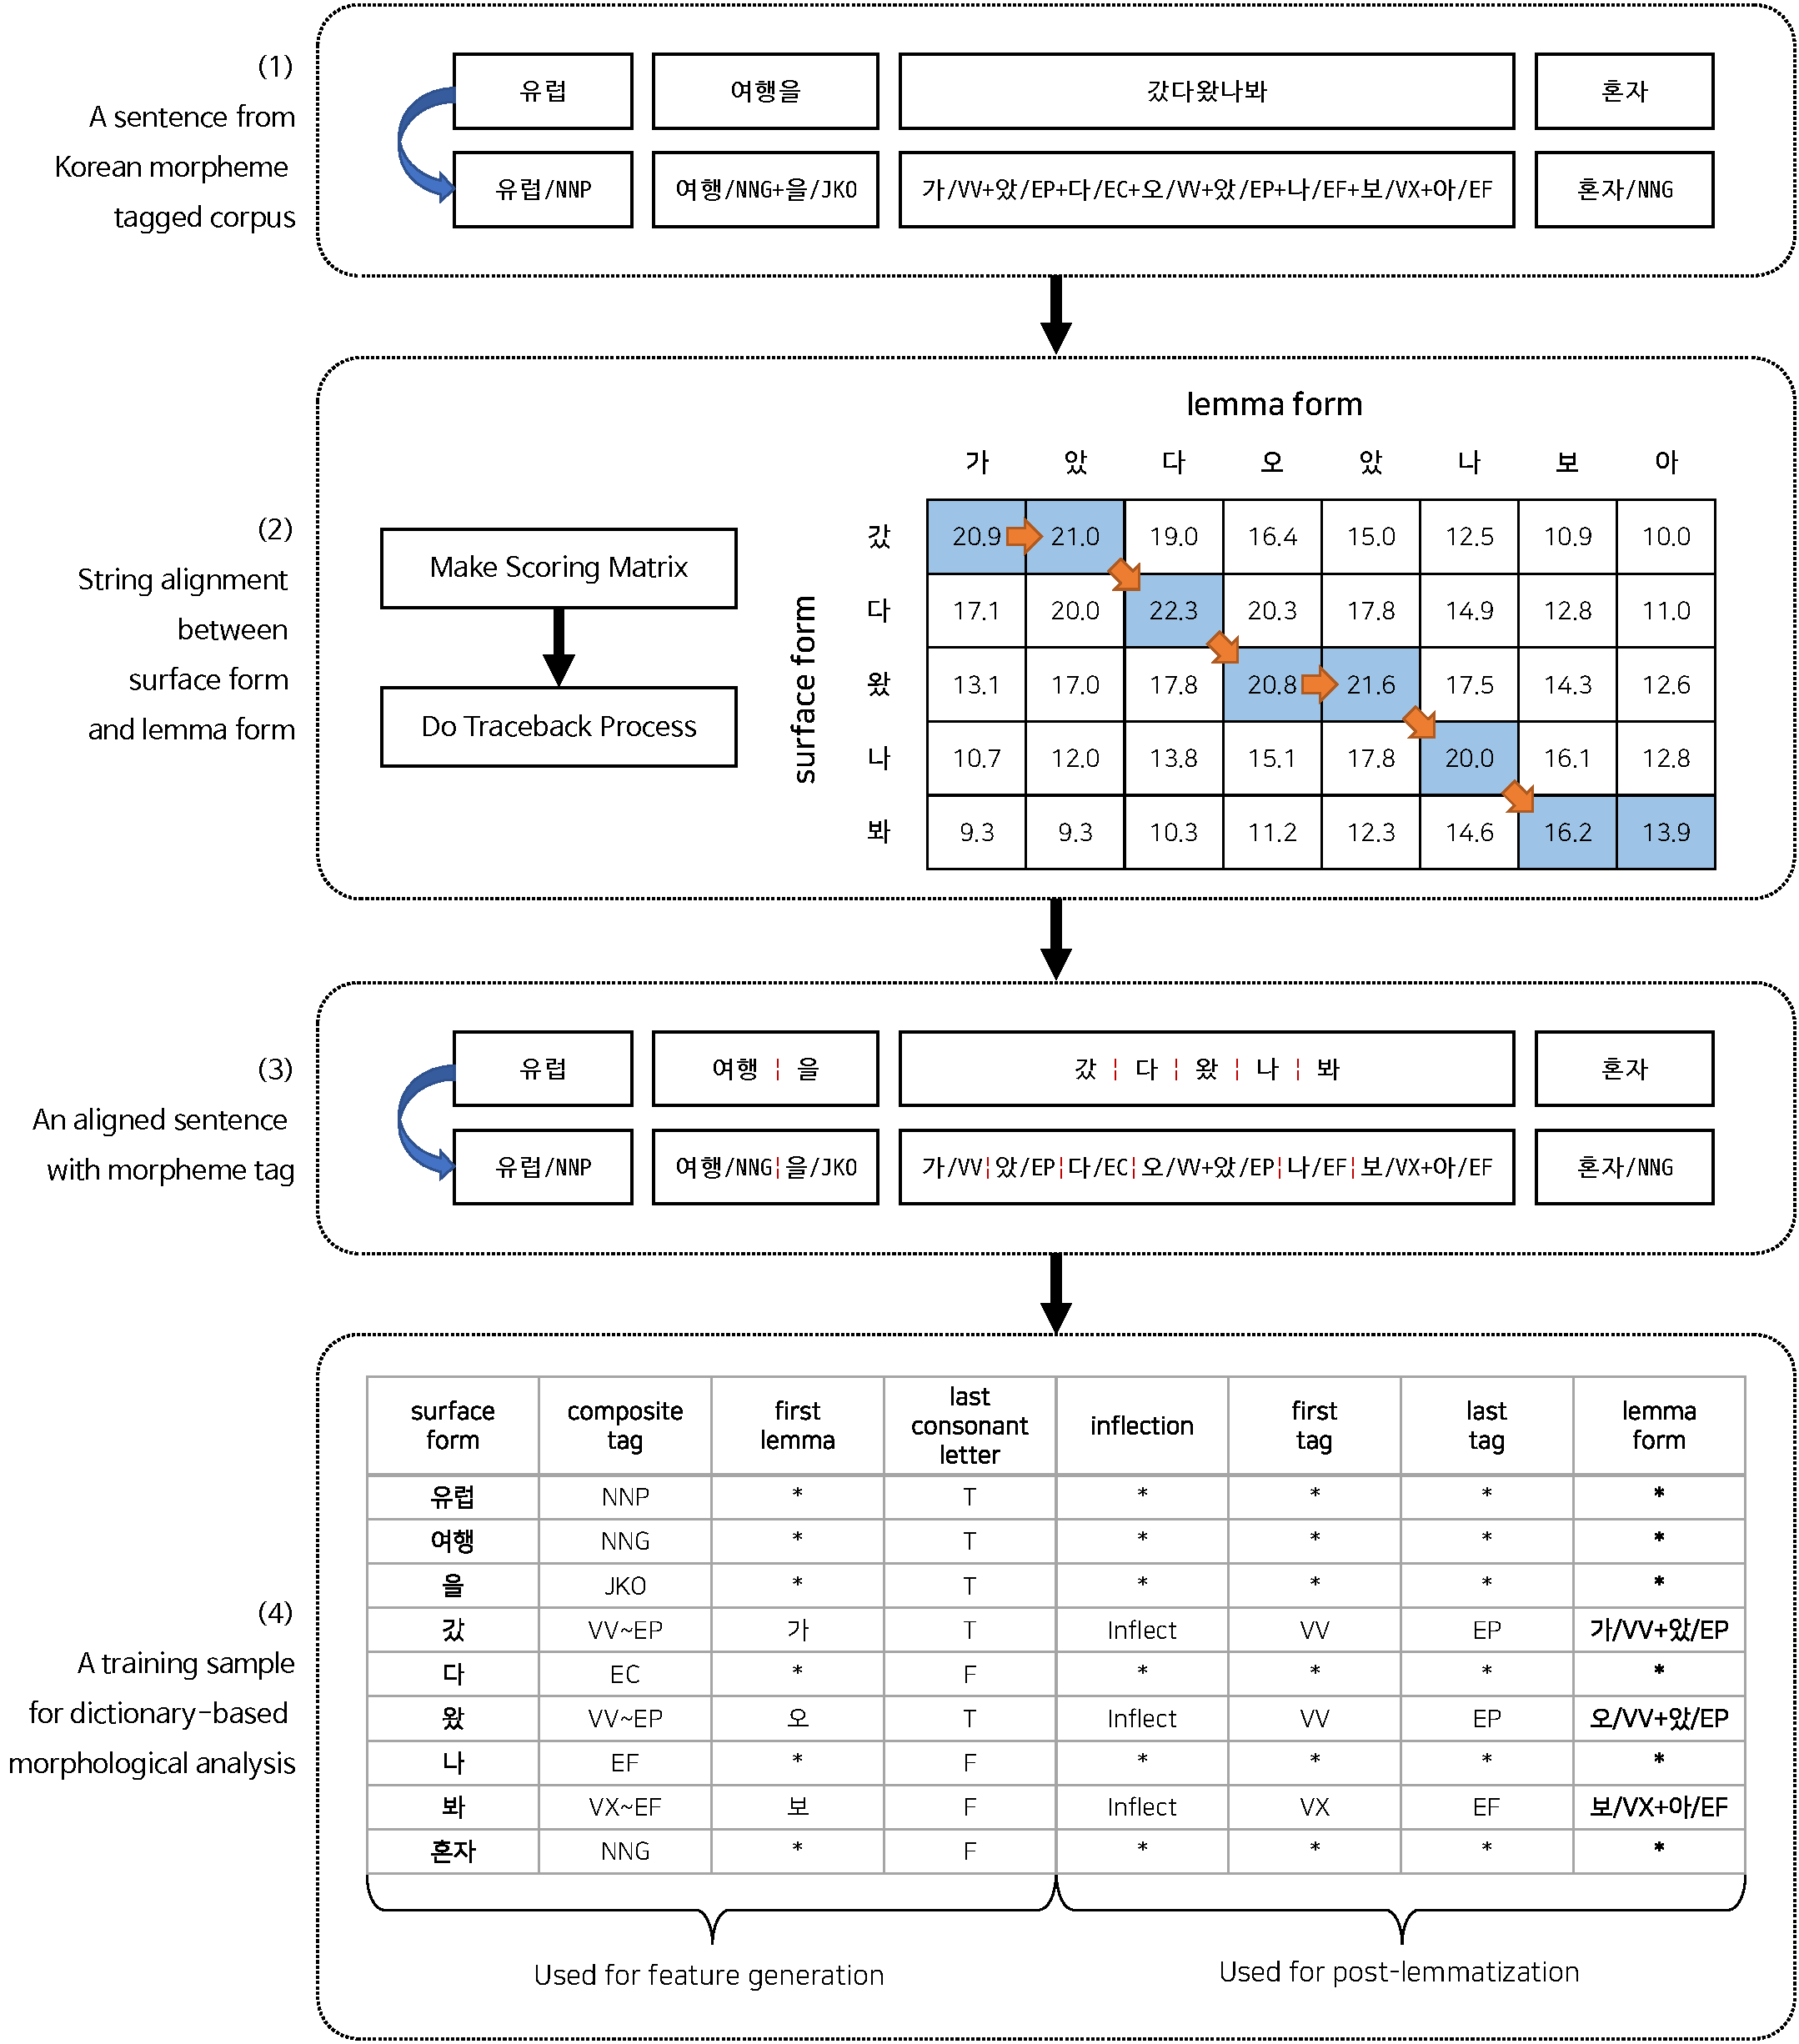
\includegraphics[width=0.9\textwidth]{fig;sample-v3}}
        \caption{Transformation of a single sentence in the Korean morpheme-tagged corpus into a single training sample}
        \label{fig:sample}
    \end{figure*}

    \subsection{Training Example Transformation}\label{subsec:training-example-transformation}

    To effectively train a dictionary-based morpheme analysis model, the morpheme-tagged corpus, typically represented in lemma form, needs transformation to include boundary information between morphemes in its surface form.
    This transformation relies on string alignment, addressing discrepancies between lemma forms and surface forms in the Korean morphological analysis corpus.

    \begin{figure*}[ht]
        \centerline{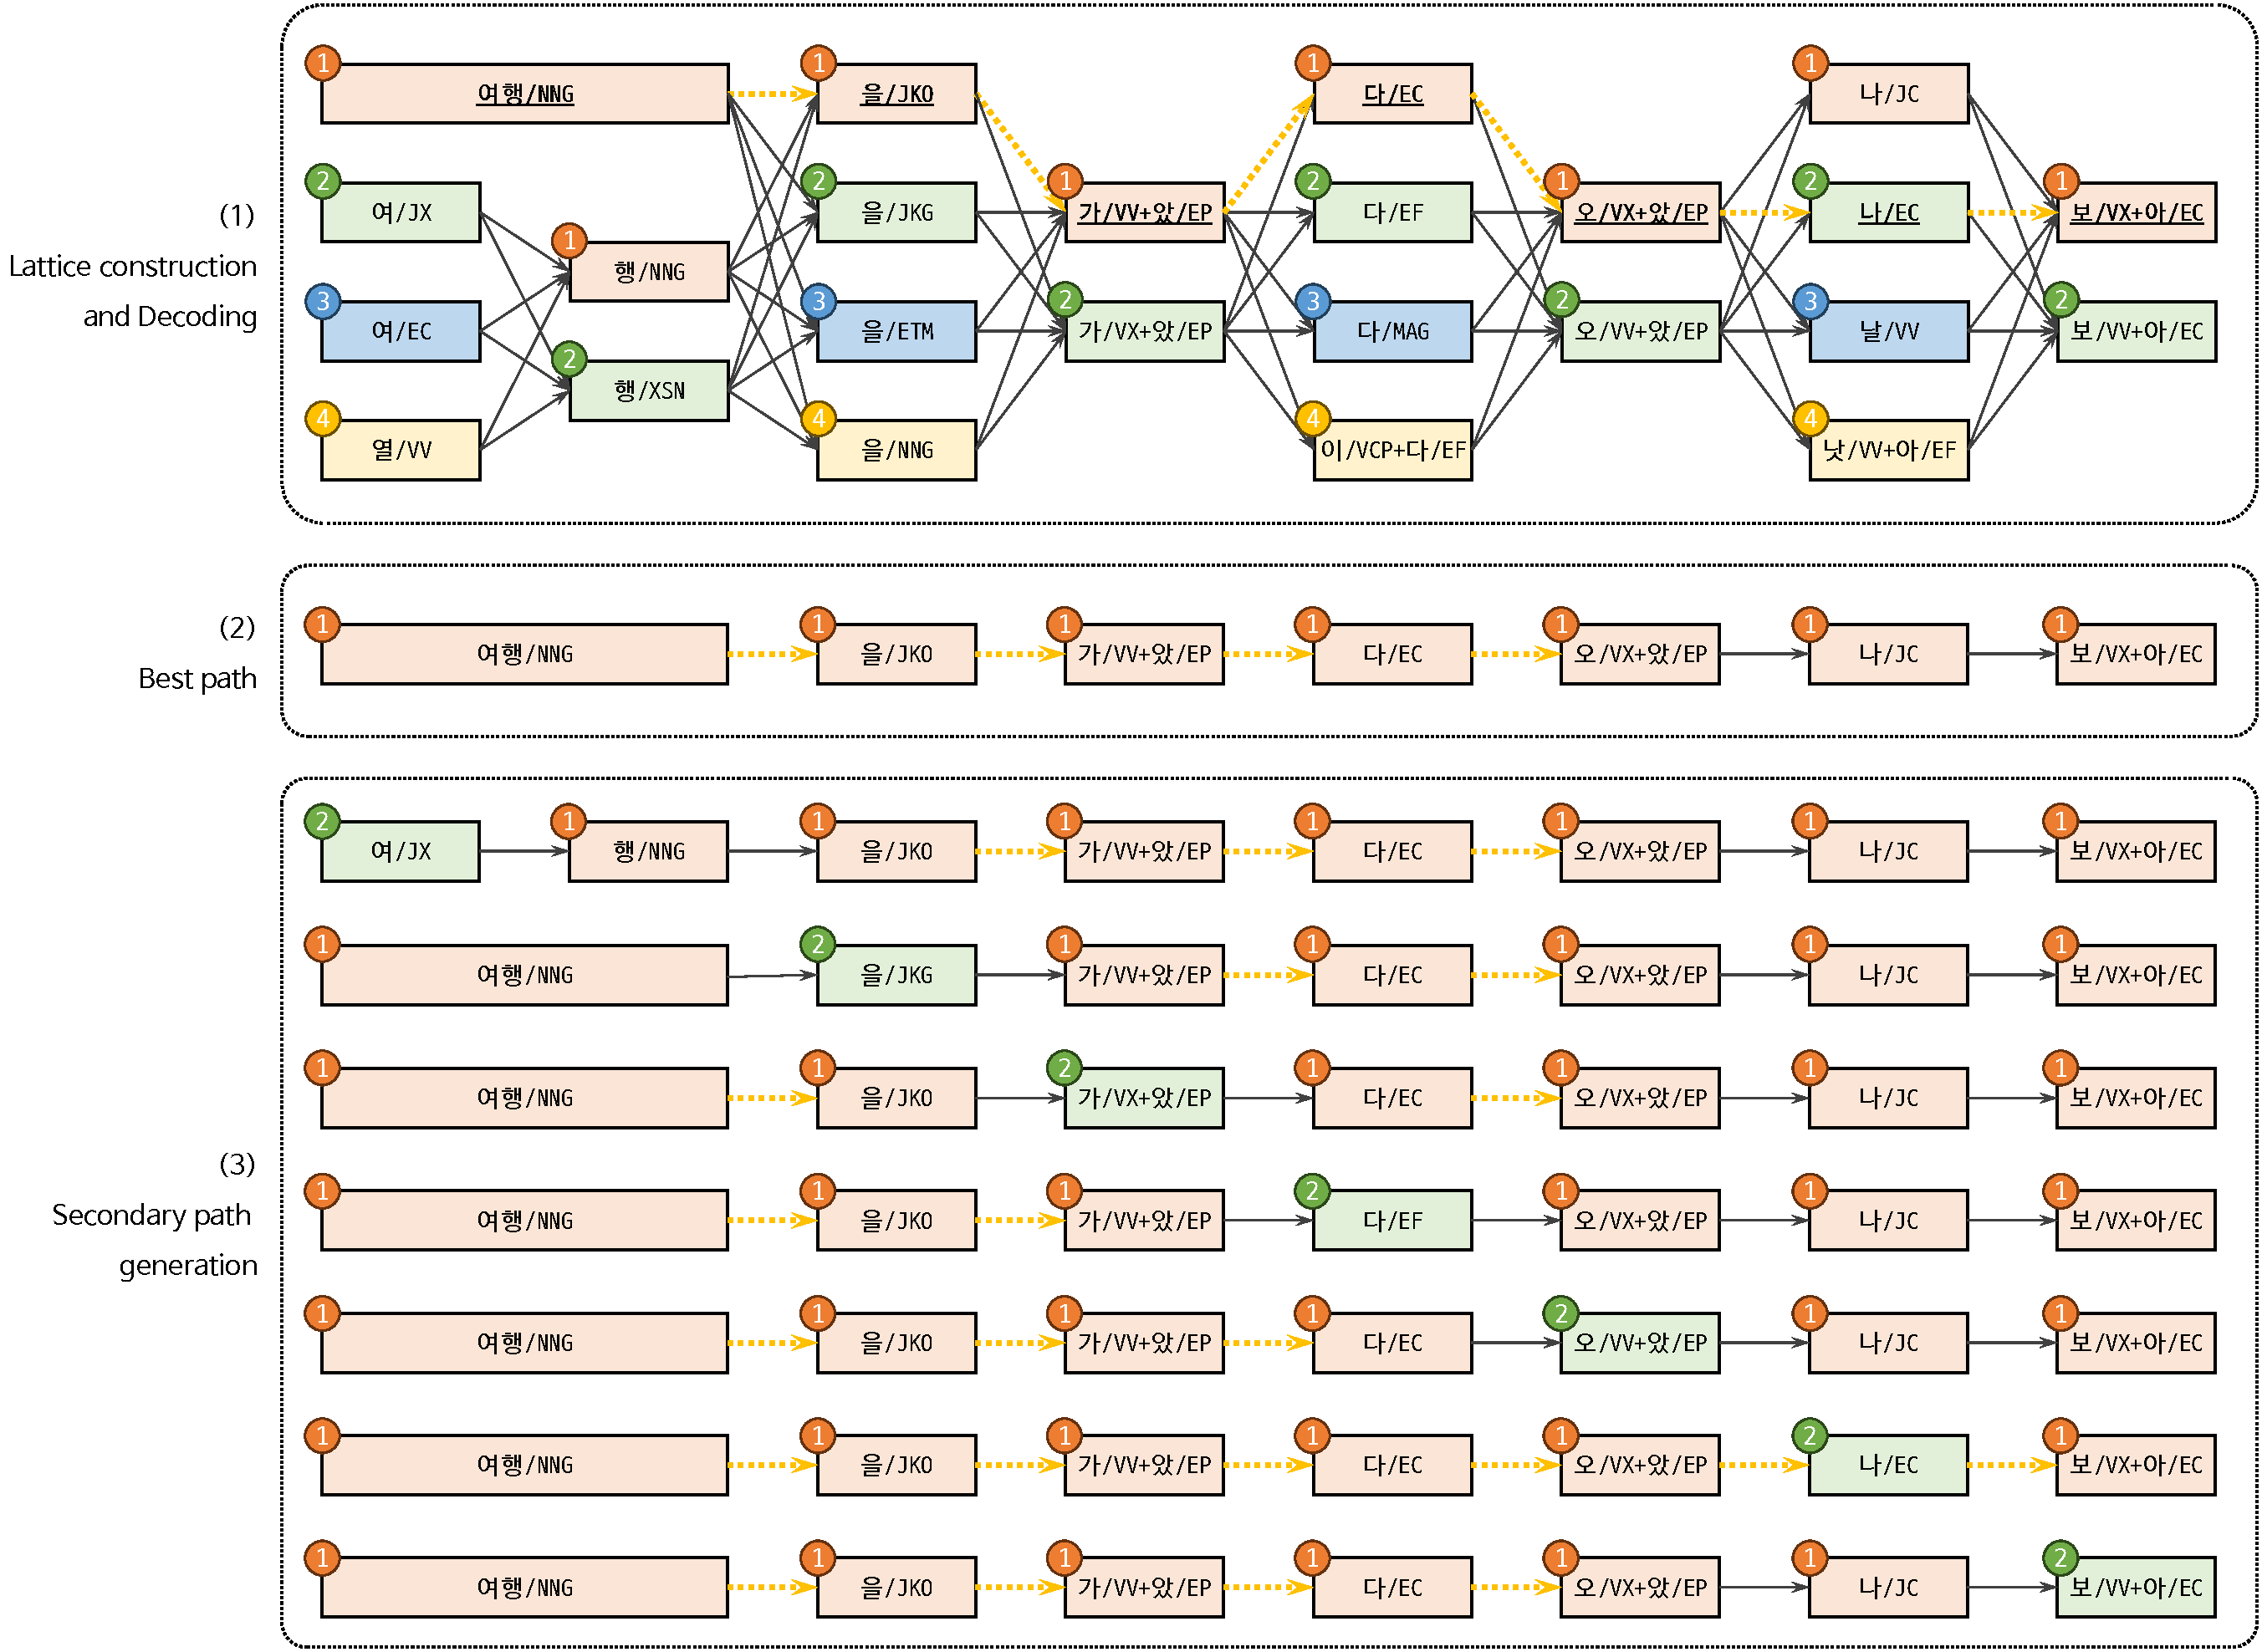
\includegraphics[width=1.0\textwidth]{fig;lattice-v3}}
        \caption{An illustrated example of a constructed lattice, the best-decoded result, and a set of the generated secondary paths. A lattice is constructed by restricting a set of nodes by morpheme lexicon, where each node is marked by its ``rank'' among a set of morphemes whose staring position are the same each other. The best path indicates the sequence of top-1 nodes in the lattice, i.e., nodes marked by the 1st rank. A secondary path is generated by replacing a top-1 node with the next top node at the same starting position, which is marked by the 2nd rank.}
        \label{fig:lattice}
    \end{figure*}

    In this study, we employed the Smith-Waterman algorithm for string alignment.
    This algorithm utilizes a scoring matrix based on the similarity of the grapheme unit of Korean letters for each word pair (as depicted in Figure~\ref{fig:sample}).
    Each aligned sentence containing a morpheme tag was then converted into a training sample tailored for dictionary-based morphological analysis.

    The resulting table in Figure~\ref{fig:sample} illustrates this process.
    Each row functions as a lexical unit, with the first four columns contributing to feature generation and the last four columns facilitating post-lemmatization.
    Leveraging the morphological corpus, a substantial number of training samples were generated following the process illustrated in Figure~\ref{fig:sample}.
    Except for the evaluation samples, the remaining sentences were employed to train the dictionary-based morphological analysis model using the CRF algorithm.
    The output of this training facilitated the calculation of costs associated with each morpheme node and the linking of two consecutive morphemes, enabling the determination of an optimal path using the Viterbi algorithm.

    \subsection{Lattice Construction and Decoding}\label{subsec:lattice-construction-and-decoding}

    In Figure~\ref{fig:lattice}, a snapshot of the lattice structure crucial to morphological analysis is presented.
    (1) displays a portion of the lattice structure formed when inputting the example sentence from Figure~\ref{fig:sample}.
    (2) illustrates the optimal path determined through the Viterbi algorithm.

    However, it's essential to note that the path predicted by the trained model might differ from the correct solution crafted by humans.
    The nodes with bold-faced and underlined text in (1) represent the correct nodes.
    The upper-left number of each node indicates the ranking of accessible nodes at each decoding point.
    Choices made at certain moments deviate from the correct solution.
    To enhance analytical performance, we have developed mechanisms that leverage deep learning, specifically BERT-based models, to correct these discrepancies.
    This integration is crucial for handling the complex morphological structures of the Korean language, as the transformer-based models provide a robust understanding of context and linguistic nuances.

    \begin{figure*}[ht]
        \centerline{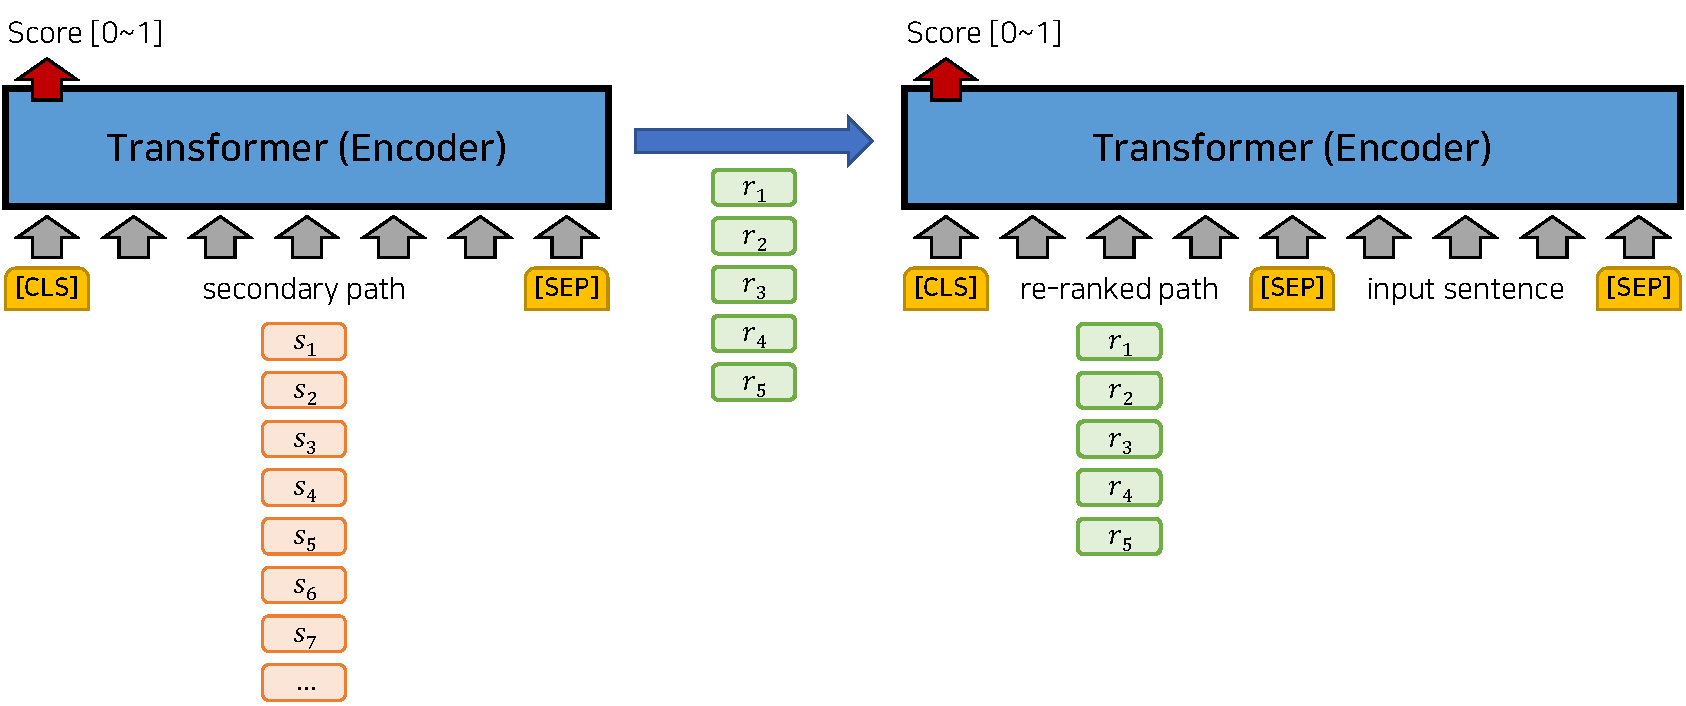
\includegraphics[width=0.9\textwidth]{fig;ranking-v2}}
        \caption{Two-stage reranking model for Korean morphological analysis. The \textit{BERT-based reranker} module takes a set of candidate secondary paths and predicts their projected scores on these BERT-encoded representations. The \textit{X-based reranker} module takes a concatenated input of a secondary path and an original input sentence and predicts its score based on the [CLS] token, where X is a variant of BERT models.}
        \label{fig:ranking}
    \end{figure*}


    \section{Reranking Model}\label{sec:reranking-model}

    While dictionary-based morphological analysis provides substantial advancements, it is not immune to instances where its optimal paths deviate from the correct solutions perceived by humans.
    To address this, we introduce a reranking model that revisits these initial results and adjusts them to enhance accuracy.
    This reranking approach involves generating multiple analyses of an input and subsequently rearranging them using a new set of criteria or models.
    Here, the BERT-based models play a pivotal role.

    \subsection{Secondary Path Generation}\label{subsec:secondary-path-generation}

    Before the reranking process initiates, multiple analyses, commonly referred to as N-best paths, of the input sentence are generated.
    This involves extracting the top N candidates from the lattice structure.
    In our study, a novel approach is introduced to produce secondary paths, as depicted in (3) of Figure~\ref{fig:lattice}, by selecting the second-best node instead of each best node constituting the path from the best-path result.
    Some of these secondary paths offered alternatives that reconciled incorrect answers with correct ones.
    Similarly, paths modified by favoring the third-best node were termed tertiary paths, and this nomenclature continued for subsequent paths.
    In our preliminary test, the secondary paths, encompassing both optimal and suboptimal paths, demonstrated coverage of the majority of correct morphological analyses, as assessed through human evaluations (refer to Table~\ref{tab:maximum-performance}).

    \subsection{BERT-based Reranking}\label{subsec:bert-based-reranking}

    Bidirectional Encoder Representations from Transformers (BERT) models~\cite{Devlin2019} have transformed numerous natural language processing tasks by comprehending the contextual nuances in which words appear in text.
    In our study, we aim to harness the capabilities of BERT to reorder the generated secondary paths.
    We assigned scores related to morphological analysis performance to the generated secondary paths and utilized them for fine-tuning a pre-trained BERT model specifically designed for Korean, enriched with a substantial amount of Korean text.
    After preliminary testing with various scoring methods on a modest scale, we found that using scores based on the degree of error, rather than accuracy-based scores, effectively widens the gap between correct and incorrect answers.

    Once the BERT model is fine-tuned and trained for the reranking task, it can predict a reranking score for each path in the secondary path list.
    This means that, taking into account the context, morphological organization, and other crucial linguistic features of the path, the model assigns a score to each path.
    Subsequently, the paths are reranked based on these scores, and the path with the highest score is selected as the optimal morphological analysis.

    \subsection{Two-stage Reranking}\label{subsec:two-stage-reranking}

    Given the complexity of the Korean language, a single reranking step does not constantly yield accurate results.
    Therefore, we propose a two-step reranking approach as described in ~\cite{Nogueira2019}.

    In the first step, we rerank the secondary paths generated using the BERT model, as outlined in Section~\ref{subsec:bert-based-reranking}.
    Subsequently, in the second step, we introduce another BERT variant optimized for a different set of linguistic features or trained on a distinct dataset.
    This enables a fine-grained re-evaluation, further refining the list and elevating more contextually accurate paths to the top.

    As shown in Figure~\ref{fig:ranking}, for a two-stage reranking model, the first stage conducts the initial reranking, taking a secondary path in morphologically tagged lemma form as input.
    The second reranking is then performed, taking the path reranked in stage 1 and the original input sentence as input.
    This approach enhances effectiveness, considering the varied input types.

    In summary, the two-stage reranking model depicted in Figure~\ref{fig:block} represents a significant advance in the approach to Korean morphological analysis.
    This model ingeniously integrates with the dictionary-based morphological analysis, where it employs a two-stage BERT-based reranking process to refine the results of the analysis.
    In the first stage, one BERT model is utilized to assess and rerank the morphological paths generated by the dictionary-based analysis.
    The second stage introduces a different BERT variant, further enhancing the reranking accuracy by considering diverse linguistic features.
    This layered approach, employing dual BERT models, is specifically designed to capture the intricacies and contextual nuances of the Korean language, addressing the challenges posed by its complex morphological structures.

    The deep learning component, particularly the BERT models, plays a pivotal role in identifying and correcting potential inaccuracies in the initial morphological analysis.
    Moreover, by evaluating morphological structures and their contextual alignment, these models significantly contribute to the accuracy of our system, especially in complex linguistic scenarios that require a deeper understanding of language context.
    The experimental setup and results, detailed in the section~\ref{sec:results}, provide crucial empirical evidence for the effectiveness of the reranking model.
    These results not only demonstrate the enhanced accuracy achieved through our innovative use of BERT models but also underscore the practical applicability of our approach in real-world Korean language processing tasks.


    \section{Experimental Results}\label{sec:results}

    Having formulated the reranking model as a theoretical framework to enhance Korean morphological analysis, our focus now shifts to empirical validation.
    This section delineates our carefully designed experimental setup, crafted to rigorously assess the performance of our model.
    Through these experiments, our goal is not only to showcase the model's accuracy but also to highlight its practical applicability in navigating the intricacies of Korean language processing.

    Our evaluation centers on the performance of the proposed deep learning-integrated dictionary-based morphological analysis method.
    The ensuing section unfolds the results of our experimental assessment, delving into the enhancements over conventional methods and elucidating the effectiveness of our reranking model.

    \subsection{Setup and Data}\label{subsec:setup-and-data}

    For our experiments, we utilized the Sejong corpus (used in ~\cite{MinJW2019, MinJW2020, MinJW2022, MinJW2018, NaSH2015, NaSH2014, NaSH2018, SongHJ2019, SongHJ2020}), UCorpus\cite{UCorpusHG}, and Everyone's Corpus\cite{EveryoneCorpus}.
    In line with previous studies for comparison purposes, the Sejong corpus underwent training using a single model without separation.
    Both UCorpus and Everyone's Corpus contributed a separate spoken corpus containing drama scripts and broadcast dialogues.
    UCorpus further categorized documents close to spoken language, organizing them into a semi-spoken corpus.
    Given the synergistic effects of training UCorpus and Everyone's Corpus simultaneously, we opted to train models separately for written and spoken language rather than segregating them by source.
    The statistics encompassing the full data for the three types of models are detailed in Table~\ref{tab:data-statistics}.
    Due to the extensive volume of UCorpus, a random selection process was employed to train the actual model.

    To prepare for training the dictionary-based morphological analysis model, we transformed this organized morphological corpus using the training-example transformation process outlined in Section~\ref{subsec:training-example-transformation}, generating samples tailored for training.

    \subsection{Evaluation Metrics}\label{subsec:evaluation-metrics}

    To assess the accuracy of the morphological analysis model, the correctness of the N-best path, and the ranking accuracy of the reranking model, we employed eojeol accuracy and morpheme F1 score as evaluation metrics.

    Eojeol accuracy measures how accurately a model identifies and processes each eojeol (a Korean linguistic unit similar to a word in English) in a sentence.
    This can be calculated as the ratio of correctly identified eojeols to the total number of eojeols in the test dataset:
    \vspace{1mm}
    \[
        \footnotesize
        \text{Eojeol Accuracy} = \frac{\text{Number of Correctly Identified Eojeols}}{\text{Total Number of Eojeols in the Test Set}}
    \]
    \vspace{0.5mm}

    Morpheme F1 score is used to evaluate a model's performance in identifying and tagging individual morphemes within an eojeol.
    It's a harmonic mean of precision and recall, where precision is the proportion of correctly identified morphemes among all identified morphemes, and recall is the proportion of correctly identified morphemes among all actual morphemes:
    \vspace{1mm}
    \[
        \footnotesize
        \text{Precision} = \frac{\text{True Positive Morphemes}}{\text{True Positive Morphemes + False Positive Morphemes}}
    \]
    \vspace{1mm}
    \[
        \footnotesize
        \text{Recall} = \frac{\text{True Positive Morphemes}}{\text{True Positive Morphemes + False Negative Morphemes}}
    \]
    \vspace{1mm}
    \[
        \footnotesize
        \text{Morpheme F1 Score} = 2 \times \frac{\text{Precision} \times \text{Recall}}{\text{Precision} + \text{Recall}}
    \]
    \vspace{0.5mm}

    In our analysis, along with conventional metrics like eojeol accuracy and morpheme F1 score, we have introduced the Error Reduction Rate (ERR) as an additional metric to quantify performance improvements.
    The ERR is especially useful in contexts where differences in raw accuracy between models are minimal.
    This metric provides a more detailed understanding of the improvements by focusing on the reduction in the proportion of errors.
    This is particularly pertinent when comparing our dictionary-based model to the syllable-based system, which is already highly tuned.
    The Error Reduction Rate (ERR) is calculated using the following formula:
    \vspace{1mm}
    \[
        \footnotesize
        \text{ERR} = \left( \frac{\text{Error Rate}_{\text{baseline}} - \text{Error Rate}_{\text{improved}}}{\text{Error Rate}_{\text{baseline}}} \right) \times 100\%
    \]
    \vspace{0.5mm}

    In this context, the error rate is defined as \(1.0 - \text{Eojeol Accuracy}\), allowing us to focus specifically on the inaccuracies in eojeol recognition.

    By incorporating ERR into our evaluation, we aim to provide a more nuanced understanding of the improvements made by our proposed method.
    In some cases, the raw accuracy figures may be close, making it challenging to discern the significance of improvements.
    ERR helps to highlight the relative improvement in terms of error reduction, offering a clearer comparison between the models and underscoring the advancements of our approach, even in the context of marginal gains in accuracy.


    \begin{table*}[ht]
        \caption{Performance comparison between morphological analysis systems without reranking}
        \label{tab:performance-without-reranking}
        \begin{tabular*}{500pt}{@{\extracolsep\fill}c|cccccc@{\extracolsep\fill}}
            \toprule
            \multirow{2}{*}{System}                & \multicolumn{2}{c}{Sejong}                                & \multicolumn{2}{c}{UCorpus (written)}                     & \multicolumn{2}{c}{Everyone's Corpus (written)}           \\
            \cmidrule{2-3} \cmidrule{4-5} \cmidrule{6-7}
            ~                                      & \multicolumn{1}{c}{eojeol} & \multicolumn{1}{c}{morpheme} & \multicolumn{1}{c}{eojeol} & \multicolumn{1}{c}{morpheme} & \multicolumn{1}{c}{eojeol} & \multicolumn{1}{c}{morpheme} \\
            \midrule
            \hspace{2mm}MeCab-ko                   & 89.17                      & 93.06                        & 87.88                      & 92.32                        & 87.77                      & 92.05                        \\
            \hspace{2mm}Syllable-based (written)   & 91.95                      & 95.16                        & \textbf{96.84}             & \textbf{97.97}               & \textbf{98.00}             & \textbf{98.82}               \\
            \hspace{2mm}Dictionary-based (written) & 90.99                      & 94.58                        & 96.33                      & 97.74                        & 96.85                      & 98.14                        \\
            \hspace{2mm}Dictionary-based (Sejong)  & \textbf{95.23}             & \textbf{97.08}               & 90.18                      & 94.19                        & 91.30                      & 94.79                        \\
            \toprule
            \multirow{2}{*}{System}                & \multicolumn{2}{c}{UCorpus (semi-spoken)}                 & \multicolumn{2}{c}{UCorpus (spoken)}                      & \multicolumn{2}{c}{Everyone's Corpus (spoken)}            \\
            \cmidrule{2-3} \cmidrule{4-5} \cmidrule{6-7}
            ~                                      & \multicolumn{1}{c}{eojeol} & \multicolumn{1}{c}{morpheme} & \multicolumn{1}{c}{eojeol} & \multicolumn{1}{c}{morpheme} & \multicolumn{1}{c}{eojeol} & \multicolumn{1}{c}{morpheme} \\
            \midrule
            \hspace{2mm}MeCab-ko                   & 86.85                      & 91.38                        & 81.75                      & 87.90                        & 85.28                      & 89.52                        \\
            \hspace{2mm}Syllable-based (spoken)    & \textbf{96.56}             & \textbf{97.65}               & \textbf{94.89}             & \textbf{96.76}               & \textbf{95.14}             & \textbf{96.82}               \\
            \hspace{2mm}Dictionary-based (spoken)  & 94.98                      & 96.65                        & 93.02                      & 95.71                        & 92.47                      & 94.83                        \\
            \bottomrule
        \end{tabular*}
    \end{table*}

    \begin{table*}[ht]
        \caption{Performance comparison between morphological analysis systems with two-stage reranking}
        \label{tab:performance-with-reranking}
        \begin{tabular*}{500pt}{@{\extracolsep\fill}c|cccccc@{\extracolsep\fill}}
            \toprule
            \multirow{2}{*}{System}                       & \multicolumn{2}{c}{Sejong}                                             & \multicolumn{2}{c}{UC+EC (written)}                                    & \multicolumn{2}{c}{UC+EC (spoken)}                                     \\
            \cmidrule{2-3} \cmidrule{4-5} \cmidrule{6-7}
            ~                                             & \multicolumn{1}{c}{eojeol}              & \multicolumn{1}{c}{morpheme} & \multicolumn{1}{c}{eojeol}              & \multicolumn{1}{c}{morpheme} & \multicolumn{1}{c}{eojeol}              & \multicolumn{1}{c}{morpheme} \\
            \midrule
            \hspace{2mm}MeCab-ko                          & 89.17                                   & 93.06                        & 87.83                                   & 92.19                        & 84.62                                   & 89.60                        \\
            \hspace{2mm}Syllable-based                    & 91.95                                   & 95.16                        & 97.42                                   & 98.39                        & 95.53                                   & \textbf{97.08}               \\
            \hspace{2mm}Dictionary-based (without rerank) & 95.23\footnotesize{ [+0.0\%]}           & 97.08                        & 96.59\footnotesize{ [+0.0\%]}           & 97.94                        & 93.49\footnotesize{ [+0.0\%]}           & 95.73                        \\
            \hspace{2mm}Dictionary-based (1-stage rerank) & 96.63\footnotesize{ [+29.2\%]}          & 97.84                        & 97.50\footnotesize{ [+26.7\%]}          & 98.44                        & 94.77\footnotesize{ [+19.6\%]}          & 96.62                        \\
            \hspace{2mm}Dictionary-based (2-stage rerank) & \textbf{96.87}\footnotesize{ [+34.4\%]} & \textbf{98.01}               & \textbf{97.75}\footnotesize{ [+34.1\%]} & \textbf{98.60}               & \textbf{95.56}\footnotesize{ [+31.8\%]} & \textbf{97.08}               \\
            \bottomrule
        \end{tabular*}
        \begin{tablenotes}
            \footnotesize
            \item\hspace{2mm} * The numbers in parentheses represent the Error Reduction Rate (ERR), calculated with respect to the ``Dictionary-based (without rerank)'' as the baseline.
        \end{tablenotes}
    \end{table*}

    To validate the correctness of morphological analysis results, we measured the degree of agreement with human annotations on the corpus.
    However, due to slight differences in criteria and annotation styles among annotators labeling various corpora, including the comparison with the MeCab-ko system, the following adjustments were made:
    \begin{itemize}
        \item Sentences containing unanalyzable tags (NF, NA, and NV) were excluded from both training and evaluation.
        \item As for the tagsets, we excluded three unanalyzable tags from the 45 Sejong tagsets and used 42 tagsets.
        \item Each tag output by the MeCab-ko system was converted to the corresponding tag in the Sejong tagset.
        \item Chinese characters were converted to Chinese character tags (SH) even if they were semantically used as nouns, and consecutive Chinese characters were converted to a single morpheme.
        \item Similarly, symbol, numeral, ending, and postposition in the same tag were converted to a single morpheme, and decimal expressions were treated as a single morpheme, including the midpoint and the numbers before and after.
        \item If the first lemma letter of the ending is `[eo]', `[yeo]', or `[ah]', it is unified as `[eo]', and if it is `[eot]', `[yeot]', or `[ass]', it is unified as `[eot]'. %`어[eo]', `여[yeo]', or `아[ah]' % `었[eot]', `였[yeot]', or `았[ass]'
        \item Root tags (XR) used alone without affixes were replaced with common nouns (NNG) because they are mainly used in the Sejong corpus only.
        \item Connective endings (EC) and sentence-closing endings (EF) are not clearly defined in the tagging guidelines as mentioned in ~\cite{KimIH2010}, and there are cases where they are used interchangeably in the corpus, so we evaluated them without distinguishing them.
        \item The distinction between `[geot]' and `[geo]' is unclear in the tagging guidelines, and there are cases where they are used interchangeably in the corpus, hence, we did not distinguish between them. %`것[geot]' and `거[geo]'
        \item Compound words can be interpreted as a single morpheme or as a combination of two or more morphemes or affixes; therefore, we evaluated them without distinguishing between these interpretations.
        \item Proper nouns can also be interpreted as common nouns depending on the point of view or perspective. Human annotators have slightly different standards, and thus, they were also evaluated without distinguishing the nouns.
    \end{itemize}

    \begin{table}[ht]
        \centering
        \footnotesize
        \caption{Training Options and Software Information for Reranking Model}
        \label{tab:training-options}
        \begin{tabular}{|p{24mm}|p{25mm}|p{25mm}|}
            \hline
            ~                     & \textbf{First-Stage}                & \textbf{Second-Stage}                                        \\ \hline
            Input Type            & Only Morphological Analysis Results & First Morphological Analysis Results and Original Input Sentences \\ \hline
            Max Sequence Length   & 384                                 & 512                                                               \\ \hline
            Minibatch Size        & 120                                 & 40                                                                \\ \hline
            Training Epochs       & 5                                   & 7                                                                 \\ \hline
            Devices Used          & \multicolumn{2}{l|}{4 GPUs}                                                                             \\ \hline
            Distribution Strategy & \multicolumn{2}{l|}{ddp}                                                                                \\ \hline
            FP Precision          & \multicolumn{2}{l|}{16-bit}                                                                             \\ \hline
            Learning Rate         & \multicolumn{2}{l|}{$2 \times 10^{-5}$}                                                                 \\ \hline
            LR Scheduler          & \multicolumn{2}{l|}{ExponentialLR (gamma=0.9)}                                                          \\ \hline
            Optimizer Type        & \multicolumn{2}{l|}{AdamW}                                                                              \\ \hline
            PyTorch               & \multicolumn{2}{l|}{version 2.0.1}                                                                      \\ \hline
            PyTorch Lightning     & \multicolumn{2}{l|}{version 2.0.6}                                                                      \\ \hline
            Transformers          & \multicolumn{2}{l|}{version 4.31.0}                                                                     \\ \hline
        \end{tabular}
    \end{table}

    \subsection{Basic Performance}\label{subsec:basic-performance}

    In our preliminary analysis, we compared the outcomes of our newly developed dictionary-based morphological analysis model, as detailed in Section~\ref{sec:morphological-analysis-model}, against the existing MeCab system and the syllable-based morphological analysis system.
    The findings, presented in Table~\ref{tab:performance-without-reranking}, demonstrate that our dictionary-based model surpasses the MeCab system in terms of accuracy.
    This indicates the effectiveness of our approach, which relies solely on a corpus-driven methodology without external dependencies like dictionaries or rule sets.

    However, when it comes to the syllable-based system, our model did not achieve comparable performance.
    The syllable-based system, as outlined in the research by Lee et al.~\cite{LeeCH2016}, has been substantially enhanced through the use of a pre-analyzed dictionary.
    This integration has significantly elevated its performance, allowing for more accurate handling of various linguistic elements.
    The system's ability to excel in different evaluation sets can be attributed to this comprehensive approach that combines extensive training corpora with meticulously crafted dictionaries and rules.

    Contrastingly, our dictionary-based system, being a recent innovation, does not utilize external resources such as pre-defined dictionaries or sets of linguistic rules.
    While this approach offers benefits like simplicity and potential adaptability, it also presents limitations in capturing the complexities and nuances of natural language that are efficiently managed by the syllable-based system.

    Additionally, our model exhibited compatibility issues between different corpora.
    The model trained on the Sejong corpus performed well when evaluated on the same corpus, but it showed a decline in performance when applied to other datasets.
    This points to the need for a more diverse and comprehensive training dataset to improve the model's generalizability.

    In summary, while our dictionary-based model marks an advancement in morphological analysis, the superior performance of the syllable-based system, especially as demonstrated in the study by Lee et al.~\cite{LeeCH2016}, highlights the effectiveness of combining training corpora with additional linguistic resources.
    Future enhancements to our model could involve integrating aspects of the syllable-based approach, such as incorporating rule-based methods or additional dictionaries, to further refine its performance.

    \begin{table*}[ht]
        \caption{Comparison of performance differences with previous studies}
        \label{tab:differences-with-previous-studies}
        \begin{tabular*}{500pt}{@{\extracolsep\fill}ccc|cc@{\extracolsep\fill}}
            \toprule
            \multirow{2}{*}{Study}                & \multirow{2}{*}{Model}                          & \multirow{2}{*}{Data (train, test)}         & \multicolumn{2}{c}{Performance}                           \\
            \cmidrule{4-5}
            ~                                     & ~                                               & ~                                           & \multicolumn{1}{c}{eojeol} & \multicolumn{1}{c}{morpheme} \\
            \midrule
            Na, 2015~\cite{NaSH2015}              & CRF++, Lattice-based HMM                        & Sejong 200k, 50k sentences                  & 95.22                      & 97.21                        \\
            Lee et al., 2016~\cite{LeeCH2016}     & Structural SVM                                  & Sejong 666k, 74k eojeols                    & 96.41                      & -                            \\
            Li et al., 2017~\cite{Li2017}         & Seq2seq (GRU-based)                             & Sejong 90k, 10k sentences                   & 95.33                      & 97.15                        \\
            Na and Kim, 2018~\cite{NaSH2018}      & Lattice + HMM                                   & Sejong 200k, 50k sentences                  & 96.35                      & 97.74                        \\
            Min et al., 2019~\cite{MinJW2019}     & Seq2seq (Transition-based)                      & Sejong 200k, 50k sentences                  & 96.34                      & 97.68                        \\
            Song and Park, 2019~\cite{SongHJ2019} & Seq2seq (BiLSTM-based)                          & Sejong 200k, 50k sentences                  & 95.68                      & 97.43                        \\
            Youn et al, 2021~\cite{YounJY2021}    & Seq2seq (BERT-based)                            & Sejong 675k, 75k sentences                  & 95.99                      & 97.94                        \\
            Shin et al, 2023~\cite{ShinHJ2023}    & Transformer(Encoder) + BiLSTM                   & Sejong 769k, 87k sentences                  & 96.12                      & 97.74                        \\
            \midrule
            Proposed (without rerank)             & \multirow{3}{*}{Lattice + Transformer(Encoder)} & \multirow{3}{*}{Sejong 194k, 10k sentences} & 95.23                      & 97.08                        \\
            Proposed (1-stage rerank)             & ~                                               & ~                                           & 96.63                      & 97.84                        \\
            Proposed (2-stage rerank)             & ~                                               & ~                                           & \textbf{96.87}             & \textbf{98.01}               \\
            \bottomrule
        \end{tabular*}
    \end{table*}

    \subsection{Reranking Performance}\label{subsec:reranking-performance}

    With the integration of the BERT-based reranking model, we observed substantial performance enhancement.
    Table~\ref{tab:performance-with-reranking} illustrates that the reranking model identified a better path in a significant proportion of cases.
    The first-stage reranking exhibited a performance improvement of over 20\% compared to traditional models.
    Subsequent reranking, leveraging a distinct type of input and a different pre-trained model, further augmented the performance by more than 30\%.

    In the BERT-based reranking process described in Section~\ref{sec:reranking-model}, we evaluated the performances using three distinct pre-trained language models renowned for their effectiveness in Korean language understanding tasks: KPF-BERT, ETRI-ELECTRA, and ETRI-RoBERTa.

    \textbf{KPF-BERT}~\cite{KPF_BERT}: The Korea Press Foundation released KPF-BERT, a result of their `Language Information Resource Development Project for Media'.
    KPF-BERT is a BERT model trained on BigKinds news data owned by the Foundation.
    Unlike previous Korean BERT models primarily trained on Wikipedia and web documents, it was refined to optimize for news agencies and article utilization.
    This was achieved by training on about 40 million selected articles from the 80 million BigKinds articles spanning from 2000 to August 2021 (Vocabulary size: 36,440).

    \textbf{ETRI-ELECTRA}, \textbf{ETRI-RoBERTa}: ETRI developed and released a BERT model pre-trained on 23GB of Korean text~\cite{KorBERT}, and in 2021, an ELECTRA model trained on 31GB of Korean text incorporating Whole Word Masking technology (Vocabulary size: 33,806).
    In 2022, they developed a RoBERTa model pre-trained on 36GB of Korean text with Byte-level BPE (Byte Pair Encoding) tokenization technology (Vocabulary size: 50,032).

    Each model uses a different form of vocabulary, so we had to vary the input accordingly.
    Preliminary tests showed that two-stage reranking using the same model or input did not improve performance, but using different models and input types did.

    Training data for the reranking model comprised 190,000 sentences from the Sejong corpus, 240,000 sentences from the written language of the combined UCorpus and Everyone's corpus, and 360,000 sentences from the spoken language of the combined UCorpus and Everyone's corpus.
    Utilizing a floating-point 16-bit technique with four GPUs for distributed training significantly reduced the training time.
    The minibatch size was 120 with a maximum sequence length of 384 for the first reranking, considering only the morphological analysis results as input.
    For the second reranking, the minibatch size was 40 with a maximum sequence length of 512, as the original input sentences were given as input along with the first morphological analysis results.
    Details on other training options and software tools can be found in Table~\ref{tab:training-options}.

    Table~\ref{tab:performance-with-reranking} demonstrates that incorporating the reranking model significantly improves performance compared to no reranking.
    The error reduction rate (ERR) of the performance change from the existing dictionary-based model on eojeol accuracy is 29\%, 27\%, and 20\% for the Sejong corpus, combined written corpus, and combined spoken corpus, respectively, with the first round of reranking.
    The second round of reranking further improves the performance by increasing the rate to 34\%, 34\%, and 32\%, respectively.
    These performance improvements underscore the superiority of the dictionary-based morphological analysis model over traditional syllable-based morphological analysis systems, including those with numerous pre- and post-processing rules and dictionaries.

    \subsection{Comparison to Other Studies}\label{subsec:comparison-to-other-studies}

    The proposed transformer-based reranking technique consistently improved the results of existing morphological analysis models, showcasing its potential to enhance outcomes in the field of Korean morphological analysis (refer to Table~\ref{tab:differences-with-previous-studies}).
    Our approach opens new avenues by further refining the results of traditional machine-learning models.
    Our study utilized the same dataset from the Sejong corpus as employed in prior research ~\cite{MinJW2019, MinJW2020, MinJW2022, MinJW2018, NaSH2015, NaSH2014, NaSH2018, SongHJ2019, SongHJ2020}.

    While direct comparisons can be challenging due to minor differences in implementation conditions and evaluation criteria, our dictionary-based morphological analysis model, augmented with a reranking model, achieved performance levels comparable to those of existing research.
    As mentioned in Section~\ref{subsec:evaluation-metrics}, that evaluation standards can vary slightly across different studies.
    Additionally, the process of transforming training data might lead to varying amounts of data being removed or excluded, which could affect the precision of direct comparisons.

    Our entire morphological analysis model, including the two-stage reranking model, might not yet be optimized for real-time processing due to its computational intensity.
    The reranking process, which evaluates all secondary paths generated by the morphological analysis, demands significant computational resources and power.
    This requirement, combined with the need for rapid response times in real-time applications, could introduce latency that may not be acceptable for certain use cases.
    The current design of our system may not efficiently manage continuous data streams and the high throughput necessary for real-time operation, potentially leading to noticeable delays for users.

    However, we recognize the potential for performance enhancement.
    By using cases where ranks are altered through the reranking model as feedback for the dictionary-based morphological analysis model, it becomes feasible to achieve near-improved morphological analysis performance.
    This enhanced dictionary-based model could then be re-input into the reranking model, creating a feedback loop that fosters iterative improvements in the overall morphological analysis process.
    This approach not only demonstrates the effectiveness of our model in a controlled environment but also indicates the potential for broader applicability and adaptability across various types of Korean text datasets.


    \section{Related Work}\label{sec:related-work}

    In recent years, Korean morphological analyses have witnessed a diverse range of methodologies~\cite{KwonHC1991, LeeDG2009, ShimKS2011, LeeJS2011, ShinJC2012, LeeCK2013, NaSH2014, NaSH2015, HwangHS2016, KimHM2016, ChungES2016, LeeCH2016, Li2017, NaSH2018, KimSW2018, ChoiYS2018, MinJW2018, MinJW2019, KimHM2019, SongHJ2019, MinJW2020, SongHJ2020, ChoiYS2020, HwangHS2020, KimHJ2021, YounJY2021, MinJW2022, KimJM2022, ShinHJ2023}.
    The agglutinative nature of the Korean language poses challenges that have inspired researchers to devise innovative solutions, laying the foundation for future investigations.
    Table~\ref{tab:overview-of-recent-korean-morphological-analysis-methods} offers a succinct comparison of the methodologies and key concepts from relevant studies, both directly and indirectly related to this research.
    This table provides a brief overview of the various approaches to morphological analysis.

    \begin{table}[ht]
        \centering
        \footnotesize % OR use \tiny, \small, \footnotesize, \scriptsize
        \caption{Overview of Recent Korean Morphological Analysis Methods}
        \label{tab:overview-of-recent-korean-morphological-analysis-methods}
        \begin{tabular}{|p{10mm}|p{24mm}|p{40mm}|}
            \hline
            \textbf{Study}                        & \textbf{Methodology}                                   & \textbf{Key Concepts}                                                                                             \\
            \hline
            Na et al., 2014~\cite{NaSH2014}       & Lattice-based Discriminative Approach                  & Lattice creation from a lexicon, morpheme connectivity, path optimization in morpheme lattice, POS tagging.       \\
            \hline
            Na, 2015~\cite{NaSH2015}              & Two-stage Discriminative Approach using CRFs           & Statistical morphological analysis, CRF-based morpheme segmentation and POS tagging, full sentence application.   \\
            \hline
            Na and Kim, 2018~\cite{NaSH2018}      & Phrase-based Model with CRFs                           & Phrase-based processing units, CRF integration for morpheme segmentation and POS tagging, noise-channel modeling. \\
            \hline
            Shim, 2011~\cite{ShimKS2011}          & Syllable-based POS Tagging with CRFs                   & Syllable-based tagging, efficiency in label assignment, morphological analysis bypass.                            \\
            \hline
            Lee, 2013~\cite{LeeCK2013}            & Joint Model with Structural SVM                        & Word spacing and POS tagging joint modeling, error propagation reduction, structural SVM application.             \\
            \hline
            Lee et al., 2016~\cite{LeeCH2016}     & Hybrid Algorithm with Pre-analyzed Dictionary          & Syllable-based POS tagging, integration of pre-analyzed dictionary and machine learning, CRF application.         \\
            \hline
            Kim et al., 2016~\cite{KimHM2016}     & POS Tagging with Bi-LSTM-CRFs                          & Syllable pattern input, bi-directional LSTM and CRF for POS tagging, morpheme ambiguity handling.                 \\
            \hline
            Li et al., 2017~\cite{Li2017}         & Sequence-to-Sequence Model with Convolutional Features & Seq2seq model with convolutional features for morphological analysis, POS tagging.                                \\
            \hline
            Kim and Choi, 2018~\cite{KimSW2018}   & Integrated Model with Bidirectional LSTM-CRF           & Bidirectional LSTM and CRF for word spacing and POS tagging, syllable-based approach.                             \\
            \hline
            Choi and Lee, 2018~\cite{ChoiYS2018}  & Reranking Model with Seq2Seq Outputs                   & Seq2Seq model reranking, morpheme-unit embedding, n-gram based morpheme reordering.                               \\
            \hline
            Min et al., 2019~\cite{MinJW2019}     & Neural Transition-based Model                          & End-to-end neural transition-based learning, morpheme segmentation, sequence-to-sequence POS tagging.             \\
            \hline
            Kim et al., 2019~\cite{KimHM2019}     & Syllable Distribution Patterns with Bi-LSTM-CRF        & Utilization of syllable distribution, Bi-LSTM-CRF for morphological analysis and POS tagging.                     \\
            \hline
            Song and Park, 2019~\cite{SongHJ2019} & Tied Sequence-to-Sequence Multi-task Model             & Multi-task learning for morpheme processing and POS tagging, pointer-generator and CRF network integration.       \\
            \hline
            Song and Park, 2020~\cite{SongHJ2020} & Two-step Korean POS Tagger with Encoder-Decoder        & Encoder-decoder architecture for morpheme generation, sequence labeling for POS tagging.                          \\
            \hline
            Youn and Lee, 2021~\cite{YounJY2021}  & Two-step Deep Learning-based Pipeline Model            & Deep learning sequence-to-sequence models, BERT for morpheme restoration and POS tagging.                         \\
            \hline
            Shin and Lee, 2023~\cite{ShinHJ2023}  & Syllable-Based Multi-POSMORPH Annotation               & Syllable distribution patterns, Multi-POSMORPH tagging, Transformer encoder, BiLSTM usage.                        \\
            \hline
        \end{tabular}
    \end{table}

    \subsection{Traditional Dictionary-based Approaches}\label{subsec:traditional-dictionary-based-approaches}
    In the initial stages of Korean morphological analysis, the predominant methods leaned heavily on rule- and dictionary-based approaches~\cite{KwonHC1991}.
    These methodologies relied on predefined sets of linguistic rules or extensive dictionaries to identify morphemes and assign parts of speech.
    One notable advantage of this approach is its deterministic nature, often resulting in high accuracy when the input text aligns closely with the utilized rules or dictionaries.
    However, scalability and updates pose challenges, especially given the continuous evolution of language and the introduction of new words.
    The dynamic nature of language, particularly in the Internet age, has rendered the maintenance of comprehensive dictionaries a labor-intensive task.

    \subsection{Syllable-unit Morphological Analysis}\label{subsec:syllable-unit-morphological-analysis}
    To address the drawbacks of dictionary dependence, syllable-by-syllable morphological analysis has emerged as an alternative~\cite{ShimKS2011, LeeCK2013, LeeCH2016, KimHM2016, Li2017, KimSW2018, ChoiYS2018, MinJW2019, KimHM2019, SongHJ2019, SongHJ2020, YounJY2021, ShinHJ2023}.
    This approach involves either tagging each syllable and then applying a base-form restoration dictionary~\cite{ShimKS2011, LeeCH2016} or tagging the syllable with the base form already restored~\cite{YounJY2021}.
    However, a notable drawback is the difficulty in accurately identifying morpheme boundaries.
    Additionally, as the sequences increase in length, the system faces increasing challenges in comprehending long-term contextual data.

    \subsection{Recent Deep Learning Approaches}\label{subsec:recent-deep-learning-approaches}
    The incorporation of deep learning into Korean morphological analysis has brought significant advancements to the field.
    Existing deep learning methods typically employ architectures like Bidirectional Long Short-Term Memory (Bi-LSTM) networks, Convolutional Neural Networks (CNNs), and Transformer-based models.
    These approaches focus on understanding language context and sequence, utilizing the ability of these models to capture long-range dependencies and intricate patterns in text data.
    For example, Bi-LSTM-CRF models, extensively used for sequence labeling in morphological analysis, leverage LSTM's capacity to remember long-term dependencies and CRF's proficiency in sequence prediction.

    In contrast, our method innovatively integrates the reranking concept with BERT-based models for Korean morphological analysis.
    Unlike traditional deep learning methods that primarily use sequence-to-sequence or sequence labeling approaches, our method generates suboptimal paths using dictionary-based techniques, which are then reranked by BERT models.
    This dual approach, leveraging BERT's contextual understanding, allows for a more detailed and accurate morphological analysis.
    The distinction of our approach lies in its ability to address the complexities of the Korean language.
    By generating and reranking suboptimal paths, our method can identify and rectify anomalies that standard deep learning models may miss.
    This innovative strategy combines the precision of dictionary-based methods with the contextual comprehension of BERT models, marking a significant advancement in the field, especially for languages with intricate morphological structures like Korean.

    \subsection{Integrating Dictionary-based and Deep Learning Approaches}\label{subsec:integrating-dictionary-based-and-deep-learning-approaches}
    Tokenization, a fundamental process in NLP deep learning models, involves breaking down text into smaller units and converting these tokens into vectors for computational processing.
    In the case of Korean, with its complex morphological characteristics, tokenization that respects morpheme boundaries is crucial.
    This approach not only accurately captures the linguistic nuances of Korean but also enhances the overall performance of deep learning models.
    This is particularly critical given the agglutinative nature of Korean, where words are formed by combining morphemes with different semantic and syntactic information.

    The combination of dictionary-based morphological analysis methods and deep learning approaches used by MeCab~\cite{MeCab}, a fast and lightweight morphological analyzer for Korean and Japanese tokenization, proves to be valuable in this context.
    The dictionary-based morphological analysis employs a model trained with CRFs to form a lattice structure as in ~\cite{Kudo2004, NaSH2014, NaSH2018}, identifying the optimal path for morphological analysis.
    While this method provides a certain level of accuracy and speed, it falls short of the high accuracy achieved by modern deep learning.

    The research aimed to bridge this gap by effectively combining dictionary-based morphological analysis methods with the contextual understanding capabilities of deep learning.
    Future research should further refine these hybrid methods, exploring the potential of end-to-end models that seamlessly integrate the strengths of traditional dictionary-based analysis with the adaptive capabilities of deep learning.
    This direction holds the promise of significant advances in morphological analysis, pushing the boundaries of Korean language processing even further.


    \section{Conclusion}\label{sec:conclusion}

    This study represents a significant advancement in Korean morphological analysis, seamlessly integrating traditional dictionary-based techniques with state-of-the-art deep learning methodologies.
    Our findings reveal that relying solely on dictionary-based morphological analysis may not surpass the efficacy of some existing models, but the incorporation of a BERT-based reranking system notably enhances accuracy, establishing a new standard in this domain.

    While the performance improvement comes with increased computational demand, the introduced methodology provides a promising avenue for continuous enhancement.
    This innovative fusion of classical dictionary approaches and cutting-edge machine-learning methodologies opens the door to groundbreaking advancements in the intricate and multifaceted domains of Korean linguistic processing.

    Future endeavors in this domain should prioritize the refinement of this harmonious integration to achieve even higher precision in morphological analysis while optimizing computational efficiency.
    Moreover, our observations suggest the potential use of a probabilistic model to identify areas prone to inaccuracies, enabling the retrieval of more accurate interpretations from a narrower candidate pool.
    The parallels between this initiative and the challenges of translation quality estimation indicate that insights from the latter can further bolster the efficacy of our approach.


    \section*{Acknowledgments}
    This work was supported by Institute of Information \& Communications Technology Planning \& Evaluation(IITP) grant funded by the Korea government(MSIT) (RS-2023-00216011, Development of artificial complex intelligence for conceptually understanding and inferring like human)


    \bibliography{references}

\end{document}
